\documentclass[10pt,a4paper]{article}
\usepackage[T1]{fontenc}
\usepackage[utf8]{inputenc}
\usepackage{lmodern}
\renewcommand{\familydefault}{\sfdefault}
\usepackage[margin=1.3cm,top=0.7cm,bottom=0.6cm]{geometry}
\usepackage{amsmath,amssymb}
\usepackage{graphicx}
\usepackage{xcolor}
\usepackage{ragged2e}
\usepackage{fontawesome5}
\usepackage{fancyqr}
\usepackage{enumitem}
\usepackage[most]{tcolorbox}
\usepackage[hidelinks]{hyperref}

\graphicspath{{assets/}}
\pagestyle{empty}
\setlength{\parindent}{0pt}
\setlist{nosep, leftmargin=1.2em, topsep=0.1em, itemsep=0.1em}

% --------------------------------------------------
% Colours: moloch theme + semantic colours of the deck
% --------------------------------------------------
\definecolor{mDarkTeal}{HTML}{23373B}
\definecolor{mLightBrown}{HTML}{EB811B}
\definecolor{robotBlue}{HTML}{4C78A8}
\definecolor{cheeseGold}{HTML}{C9A100}
\definecolor{goalPink}{HTML}{D6409F}
\definecolor{goalGreen}{HTML}{3E9B4F}
\definecolor{beliefPurple}{HTML}{8E5BA8}
\definecolor{tellerTeal}{HTML}{2A9D8F}
\definecolor{borgesRed}{HTML}{B5443A}

\newcommand{\robot}[1]{\textcolor{robotBlue}{#1}}
\newcommand{\cheese}[1]{\textcolor{cheeseGold!85!black}{#1}}
\newcommand{\pink}[1]{\textcolor{goalPink}{#1}}
\newcommand{\green}[1]{\textcolor{goalGreen}{#1}}
\newcommand{\belief}[1]{\textcolor{beliefPurple}{#1}}
\newcommand{\teller}[1]{\textcolor{tellerTeal}{#1}}
\newcommand{\borges}[1]{\textcolor{borgesRed}{#1}}
\newcommand{\alert}[1]{\textcolor{mLightBrown}{#1}}
\newcommand{\Prob}{\mathrm{P}}
\newcommand{\note}[1]{{\footnotesize\color{black!70}#1}}

% moloch-style filled blocks
\tcbset{mbase/.style={
  enhanced, sharp corners, boxrule=0pt, frame hidden,
  colback=mDarkTeal!6, colbacktitle=mDarkTeal!14,
  fonttitle=\bfseries\small, fontupper=\small\RaggedRight,
  left=4pt, right=4pt, top=3pt, bottom=3pt,
  toptitle=1.5pt, bottomtitle=1.5pt, before skip=0pt, after skip=3.5pt}}
\newtcolorbox{mblock}[2][]{mbase, coltitle=mDarkTeal, title={#2}, #1}
\newtcolorbox{malert}[2][]{mbase, coltitle=mLightBrown!75!black, title={#2}, #1}

\begin{document}

% ==================================================
% Header bar
% ==================================================
\begin{tcolorbox}[enhanced, sharp corners, boxrule=0pt, frame hidden,
  colback=mDarkTeal, coltext=white, left=8pt, right=8pt, top=6pt, bottom=6pt, after skip=1pt]
\begin{minipage}[c]{0.82\linewidth}
{\LARGE\bfseries Storytelling as Inverse Inverse Planning}\\[0.25em]
{\small Chandra, Li, Tenenbaum \& Ragan-Kelley (2023), read with Borges, \emph{The Garden of Forking Paths} (1941)}\\[0.25em]
{\footnotesize Aldo Costa, Jonas Ingenhaag \quad\textbullet\quad Master-Seminar: Theory of Mind, HHU \quad\textbullet\quad 21.01.2027}
\end{minipage}\hfill
\begin{minipage}[c]{0.15\linewidth}
\centering
{\setlength{\fboxsep}{0.12cm}\colorbox{white}{\fancyqr[size=1.5cm, color=black, level=M]{https://github.com/Eyecatch3r/storytelling-inverse-inverse-planning-seminar}}}\\[0.1em]
{\tiny Notes and slides}
\end{minipage}
\end{tcolorbox}
{\color{mLightBrown}\rule{\linewidth}{1.2pt}}

\vspace{0.4em}
\begin{malert}{\faLightbulb\ In one sentence}
A storyteller plans for the \belief{audience's beliefs}, not for the characters' goals: it chooses actions so that the audience's inferences, modelled as Bayesian theory of mind, follow a designed path.
\end{malert}

% ==================================================
% Two columns
% ==================================================
\begin{minipage}[t]{0.49\linewidth}\vspace{0pt}

\begin{mblock}{\faFilm\ Motivation}
Viewers see agents with goals in simple moving shapes (Heider \& Simmel, 1944). A rational planner reaches its goals, but an efficient path leaves no doubt, so it has no suspense and no irony. Kukkonen (2014): a story is a ``probability design'' of the reader's beliefs.
\end{mblock}

\begin{mblock}{\faBrain\ Three levels}
\begin{tabular}{@{}l@{\hspace{0.5em}}l@{}}
\textbf{Planning} & goal $\rightarrow$ actions (act)\\
\textbf{Inverse planning} & actions $\rightarrow$ \belief{$\Prob(\text{goal}\mid\text{actions})$} (ToM)\\
\textbf{Inverse inverse} & \teller{objective} $\rightarrow$ actions, via an audience model\\
\end{tabular}
\end{mblock}

\begin{mblock}{\faRobot\ Audience model (Ullman et al., 2009)}
Grid world: a \robot{robot} that can push objects and a weak \cheese{cheese} (its moves succeed 60\% of the time), goal tiles \pink{pink} and \green{green}. The robot's reward includes $\rho\cdot r_{\text{cheese}}$, the cheese's reward weighted by $\rho$: $\rho>0$ helps, $\rho<0$ hinders, $\rho=0$ indifferent. The robot reasons about a cheese that reasons about the robot. An observer infers the hypothesis $H$ (both goals $G$ and $\rho$) from each action $a$ in state $s$:
\[
\belief{\Prob(H\mid s\to a)}\propto\Prob(s\to a\mid H)\,\Prob(H)
\]
\end{mblock}

\begin{mblock}{\faBullseye\ Optimizing a script}
A script $\sigma$ is a setting plus a sequence of moves and their outcomes, all optimized; $\sigma_{1:t}$ is the part seen so far. Beam search (keep the best few partial scripts) maximizes, for example,
\[
f_{\text{help}}(\sigma)=\textstyle\sum_{t}\belief{\Prob(\rho>0\mid\sigma_{1:t})}.
\]
The objective fixes no goals or positions. The optimizer finds a scene that \alert{shows} helping.
\end{mblock}

\begin{mblock}{\faExclamationTriangle\ Limits and critique}
\begin{itemize}
  \item \textbf{Paper}: scales badly; too slow for real time; emotion is future work.
  \item \textbf{Evidence} (critique, not from the paper): weak baseline; devices are one-seed demos, untested on humans. The method \emph{can} make readable scenes; it does not show that people plan this way.
  \item \textbf{Borges} (interpretation): the Chief must already hold the hypothesis ``a killing encodes a name''; one lossy report, not a full trajectory.
  \item \textbf{Ethics} (extension, not from the paper): the same machinery can deceive.
\end{itemize}
\end{mblock}

\begin{malert}{\faComments\ For discussion}
\begin{enumerate}
  \item What data would show that \emph{people} tell stories this way?
  \item Which objective $f$ makes Yu Tsun's murder score highest?
  \item Is the Chief a Bayesian inverse planner? With what prior?
  \item Could an LLM be the audience model? How to test it?
\end{enumerate}
\end{malert}

\end{minipage}\hfill
\begin{minipage}[t]{0.49\linewidth}\vspace{0pt}

\begin{mblock}{\faFlask\ Results}
\textbf{Exp.\ 1}: 98 participants, 120 animations, 15 per person. Indifference is easy (characters rarely interact); not all scenes allow helping.\\[0.3em]
{\centering
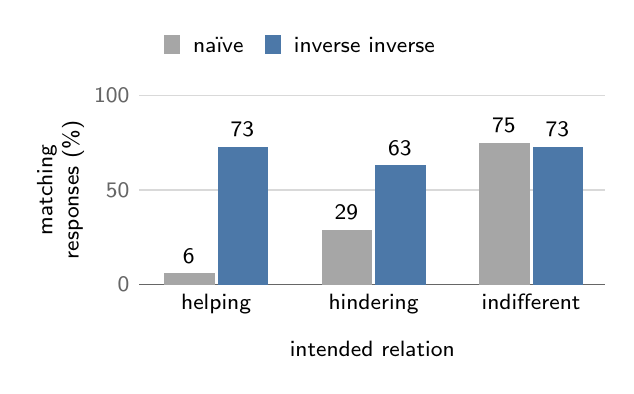
\begin{tikzpicture}[x=0.8cm, y=0.024cm, font=\footnotesize]
  \foreach \v in {0,50,100} {
    \draw[black!15] (0,\v) -- (7.4,\v);
    \node[anchor=east, black!60] at (0,\v) {\v};
  }
  \draw[black!60] (0,0) -- (7.4,0);
  \node[rotate=90, align=center] at (-1.25,50) {matching\\responses (\%)};
  \foreach \x/\n/\i/\name in {0.4/6/73/helping, 2.9/29/63/hindering, 5.4/75/73/indifferent} {
    \fill[black!35] (\x,0) rectangle ++(0.8,\n) node[above, pos=1, xshift=-0.33cm, black]{\n};
    \fill[robotBlue] (\x+0.85,0) rectangle ++(0.8,\i) node[above, pos=1, xshift=-0.33cm, black]{\i};
    \node[below] at (\x+0.82,0) {\name};
  }
  \node at (3.7,-34) {intended relation};
  \fill[black!35] (0.4,122) rectangle ++(0.25,10); \node[anchor=west] at (0.7,127) {naïve};
  \fill[robotBlue] (2.0,122) rectangle ++(0.25,10); \node[anchor=west] at (2.3,127) {inverse inverse};
\end{tikzpicture}\par}
\note{Mean of 20 animations per bar. Helping, hindering: $p<0.01$; indifferent: n.s.}\\[0.2em]
\textbf{Exp.\ 2} (``inverse inverse physics''): a hopping robot mimes pulling a heavy box. Controls: chance on same-weight pairs, 97\% on honest heavy vs.\ light. The mime is judged heavier than an honest light box (\textbf{95.7\%}) and than an honest \emph{heavy} box (\textbf{68.6\%}). \note{35 participants in the text; Fig.~4b says N = 70.}
\end{mblock}

\begin{mblock}{\faRandom\ Storytelling devices as objectives}
\begin{itemize}
  \item \textbf{Plot twist}: $\Prob(\rho>0)$ in the first half, $\Prob(\rho<0)$ in the second.
  \item \textbf{Dramatic irony}: the audience knows the cheese's goal; the robot does not and hinders by mistake.
  \item \textbf{Flashback}: append a known event to $\sigma$; find a past that makes it look helpful.
  \item \textbf{Narrative arc}: fortune rises, falls, rises; a KL penalty on belief changes keeps the goals stable; a table can fall ``from the sky'' that no character expects (deus ex machina).
\end{itemize}
\end{mblock}

\begin{mblock}{\faUserSecret\ \borges{The Garden of Forking Paths} (an interpretation)}
Yu Tsun, a German spy in England, must tell his Chief in Berlin the name of a town. He kills a stranger named Albert; the newspapers report it; the Chief understands and the town of Albert is bombed.
\begin{itemize}
  \item \textbf{Reading 1}: the murder is inverse inverse planning, with \teller{storyteller} Yu Tsun, \belief{audience} the Chief, observations = newspapers. The act is terrible in the world but is the only one that creates the belief: an extreme mime.
  \item \textbf{Reading 2}: Borges shapes the reader's belief the same way: Yu Tsun calls himself Albert's friend, then shoots (twist).
  \item \textbf{Reading 3}: Ts'ui Pen's novel takes \emph{every} branch; a storyteller keeps \emph{one} script and lets the audience infer the meaning: show, don't tell.
\end{itemize}
\end{mblock}


\end{minipage}

\vfill
{\color{black!30}\rule{\linewidth}{0.4pt}}\\[0.1em]
\note{\faLink\ Seminar: Bayesian ToM 03.12.\ \textbullet\ LLM planning 17.12.\ \textbullet\ \texttt{memo} 14.01.\ \textbullet\ false belief 29.10.\ \textbullet\ Clever Hans 05.11.\ \textbullet\ awareness 07.01.\ \textbullet\ epistemic logic 04.02.}\\[0.2em]
{\scriptsize\color{black!70}
Chandra, K., Li, T.-M., Tenenbaum, J.\,B., \& Ragan-Kelley, J. (2023). Storytelling as inverse inverse planning. \emph{Proc.\ CogSci} 45 (CC BY 4.0); code and videos: \url{https://people.csail.mit.edu/kach/a2i2p/}.
Borges, J.\,L. (1941). El jardín de senderos que se bifurcan.
Heider, F., \& Simmel, M. (1944). An experimental study of apparent behavior. \emph{Am.\ J.\ Psychol.} 57.
Ullman, T.\ et al.\ (2009). Help or hinder. \emph{NeurIPS}.
Kukkonen, K.\ (2014). Bayesian narrative. \emph{Anglia} 132.\par}

\end{document}
